\documentclass[letter]{article}
\usepackage{graphicx}
\begin{document}
\DeclareGraphicsExtensions{.png, .jpg, .pdf}

\begin{center}
	\Large\textbf{Tarea 5 Metodos Computacionales}\\
	\large\textit{Julian A. Melendez}
\end{center}
\section{Velocidad Galaxia}
\begin{figure}[h]
  \centering
    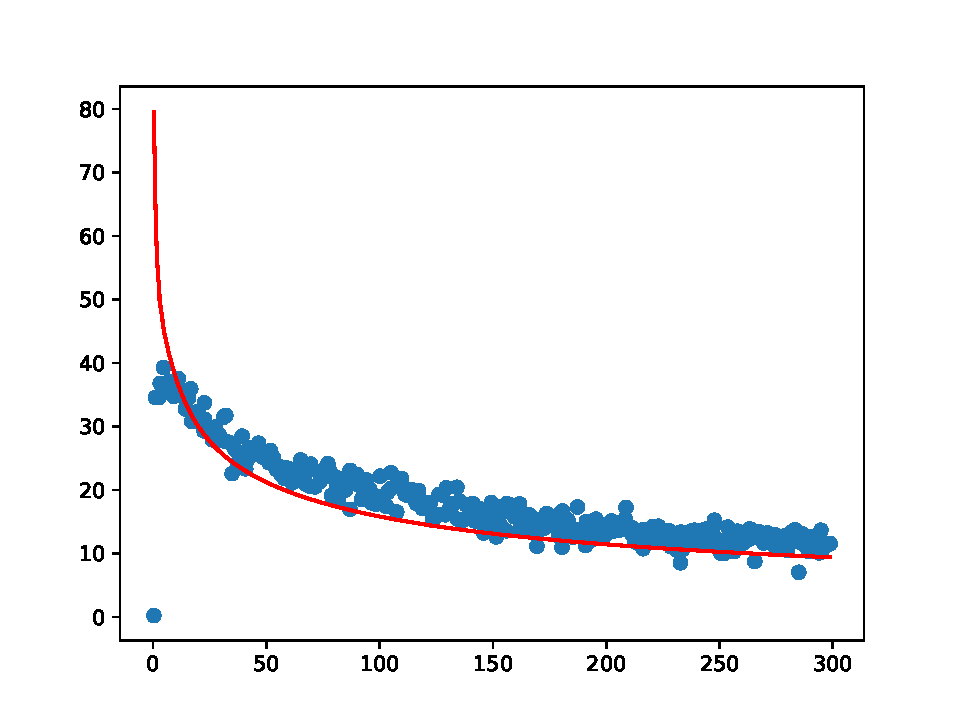
\includegraphics[width=0.9\textwidth]{Velocidad.pdf}
	\caption{Velocidades}
\end{figure}
Esta es la aproxiamcion obtenida por metodos de monte carlo



\end{document}

